\documentclass{article}
\usepackage[margin=1in]{geometry}
\usepackage{amsmath,amsthm,amssymb}
\usepackage{bbm,enumerate,mathtools}
\usepackage{tikz,pgfplots}
\usepackage{chessboard}
\usepackage[hidelinks]{hyperref}
\usepackage{multicol} % Problem 35

\newenvironment{question}{\begin{trivlist}\item[\textbf{Question.}]}{\end{trivlist}}
\newenvironment{note}{\begin{trivlist}\item[\textbf{Note.}]}{\end{trivlist}}
\newenvironment{references}{\begin{trivlist}\item[\textbf{References.}]}{\end{trivlist}}
\newenvironment{related}{\begin{trivlist}\item[\textbf{Related.}]\end{trivlist}\begin{enumerate}}{\end{enumerate}}

\begin{document}
\rating{2}{2}
We want to understand $k$-dimensional degree-$d$ B\'ezier curves with $d+1$ control points  $p_0, p_1, \dots, p_d$ in the set $\{0, 1, 2, \dots, n\}^k$: \[
  \vec{c}(t) = \sum_{i = 0}^d \binom{d}{i}t^i(1-t)^{d-i} p_i
\]
\begin{figure}[ht!]
  ~\hfill
  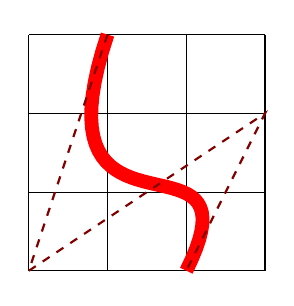
\begin{tikzpicture}
    \draw (0,0) grid (3,3);
    \draw [red, line width=5,  domain=0:1, samples=40]
      plot (
        {1*(1-\x)^3 + 0*3*\x^1*(1-\x)^2 + 3*3*\x^2*(1-\x)^1 + 2*\x^3},
        {3*(1-\x)^3 + 0*3*\x^1*(1-\x)^2 + 2*3*\x^2*(1-\x)^1 + 0*\x^3}
      );
    \draw[dashed, thick, red!50!black] (1,3)--(0,0)--(3,2)--(2,0);
  \end{tikzpicture}
  \hfill
  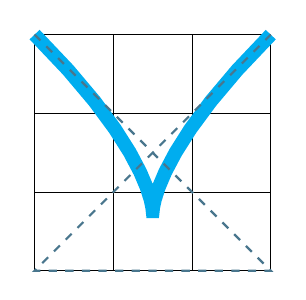
\begin{tikzpicture}
    \draw (0,0) grid (3,3);
    \draw [cyan, line width=5,  domain=0:1, samples=20]
      plot (
        {0*(1-\x)^3 + 3*3*\x^1*(1-\x)^2 + 0*3*\x^2*(1-\x)^1 + 3*\x^3},
        {3*(1-\x)^3 + 0*3*\x^1*(1-\x)^2 + 0*3*\x^2*(1-\x)^1 + 3*\x^3}
      );
    \draw[dashed, thick, cyan!50!black] (0,3)--(3,0)--(0,0)--(3,3);
  \end{tikzpicture}
  \hfill
  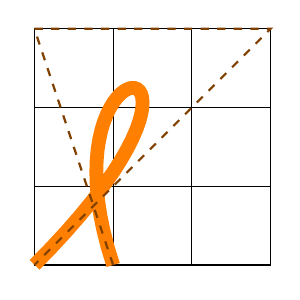
\begin{tikzpicture}
    \draw (0,0) grid (3,3);
    \draw [orange, line width=5,  domain=0:1, samples=40]
      plot (
        {1*(1-\x)^3 + 0*3*\x^1*(1-\x)^2 + 3*3*\x^2*(1-\x)^1 + 0*\x^3},
        {0*(1-\x)^3 + 3*3*\x^1*(1-\x)^2 + 3*3*\x^2*(1-\x)^1 + 0*\x^3}
      );
    \draw[dashed, thick, orange!50!black] (1,0)--(0,3)--(3,3)--(0,0);
  \end{tikzpicture}
  \hfill
  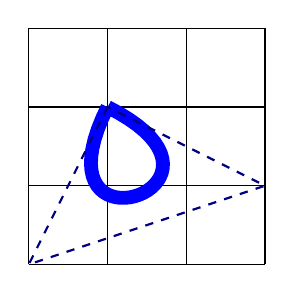
\begin{tikzpicture}
    \draw (0,0) grid (3,3);
    \draw [blue, line width=5,  domain=0:1, samples=40]
      plot (
        {1*(1-\x)^3 + 0*3*\x^1*(1-\x)^2 + 3*3*\x^2*(1-\x)^1 + 1*\x^3},
        {2*(1-\x)^3 + 0*3*\x^1*(1-\x)^2 + 1*3*\x^2*(1-\x)^1 + 2*\x^3}
      );
    \draw[dashed, thick, blue!50!black] (1,2)--(0,0)--(3,1)--(1,2);
  \end{tikzpicture}
  \hfill~
  \caption{
    Four examples of cubic B\'ezier curves with all four control points in $\{0,1,2,3\}^2$.
    The first has control points $(1,3)$, $(0,0)$, $(3,2)$, $(2,0)$.
    The second: $(0,3), (3,0), (0,0), (3,3)$.
    The third: $(1,0), (0,3), (3,3), (0,0)$.
    The fourth: $(1,2), (0,0), (3,1), (1,2)$.
  }
\end{figure}

\begin{question}
  For fixed $d$ the limit as $n \to \infty$, what is the probability of self-intersection?
\end{question}

\begin{related}
  \item How many distinct curves are there up to symmetry of the square.
  \item How many curves have a cusp?
  \item What can we say about the space of these curves when control points are instead in $[0,1]^k$? Is the set of non-self-intersecting curves connected in this setting?
  \item What are the extremal curves with respect to length, number of intersections, enclosed area, etc?
\end{related}
\begin{references}
  \item Wikipedia, ``\href{https://en.wikipedia.org/wiki/B%C3%A9zier_curve}{B\'ezier curve}.''
\end{references}

\end{document}
